\documentclass[a4paper,10pt]{article}
\usepackage[vmargin=.7cm, hmargin=1cm]{geometry}
% !TEX root = Simple-CV.tex
%-------------------------------------------------------------------------------------------------------
% Packages
%-------------------------------------------------------------------------------------------------------
\usepackage[utf8x]{inputenc}
\usepackage[T1]{fontenc}
\usepackage[spanish]{babel}
\usepackage{fontawesome}
\usepackage{datetime}
\usepackage[usenames,dvipsnames]{xcolor}
\usepackage[colorlinks=true, urlcolor=ColorTwo]{hyperref}
\usepackage{tikz}
\usepackage{hyperref}
\usepackage{setspace}
\usepackage{graphicx}
\usepackage{enumitem}
\usepackage{sectsty}
\usepackage{multicol}
\usepackage{adjustbox}
%-------------------------------------------------------------------------------------------------------
% Layout
%-------------------------------------------------------------------------------------------------------
\pagenumbering{gobble}
\renewcommand{\baselinestretch}{1.5} 
\setlength{\parindent}{0pt}

%
% Color theme
%
\definecolor{ColorOne}{RGB}{0,110,140}
\definecolor{ColorTwo}{RGB}{120,0,0}	
\definecolor{ColorThree}{RGB}{50,50,50} 	

%\sectionfont{\color{ColorOne}} 
%\subsectionfont{\color{ColorOne}} 

%
% Vertical line
%
\newcommand{\MyVerticalRule}{
	\textcolor{ColorThree}{\rule{1pt}{\textheight}}
}

%
% Update
%
\newcommand{\LastUpdate}{%
\vfill
\centering \small
\textcolor{ColorOne}{Actualizado: \monthname,~\the\year.}
}

%
% Skip
%
\newcommand{\MySkip}{
\vskip12pt
}

%
% Format hyperrefs
%
\newcommand{\myhref}[2]{%
\href{#1}{\textcolor{ColorThree}{#2}}
}
%
% Format skill bullets
%
\newcommand{\SkillBull}[1]{%
\textcolor{ColorTwo}{#1}
}


%-------------------------------------------------------------------------------------------------------

\begin{document}
\thispagestyle{empty}

%-------------------------------------------------------------------------------------------------------
% Left column
%-------------------------------------------------------------------------------------------------------
\begin{adjustbox}{valign=t}
\begin{minipage}{.44\textwidth} % Adapt width to your convenience
%----------------------------------------------------
% Please add a photo in 1x1 format
\begin{center}
\begin{tikzpicture}
	\clip (0,0) circle (2cm) node {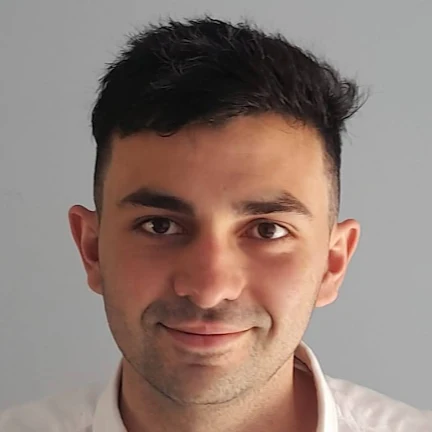
\includegraphics[width=4cm]{foto.png}};
\end{tikzpicture}

\MySkip % See MySetup.tex file

%----------------------------------------------------
{\LARGE \bfseries Renzo Zagarra Saez}

\MySkip % See MySetup.tex file

22 de Enero, 1999\\
Mendoza - Argentina\\

\MySkip %See MySetup.tex file

\textcolor{ColorThree}{\faEnvelopeO} 
\myhref{mailto:renzozagarrasaez@gmail.com}{renzozagarrasaez@gmail.com} \\

\textcolor{ColorThree}{\faGithub} 
\myhref{https://github.com/RenzoZS}{https://github.com/RenzoZS}

\textcolor{ColorThree}{\faLinkedin}
\myhref{https://www.linkedin.com/in/renzo-zagarra-saez-b086311ba/}{Renzo Zagarra Saez}

\end{center}

%----------------------------------------------------
\section*{Sobre mí}

Soy físico, me gusta entender las cosas en profundidad y de la manera
más sencilla posible. Me gusta compartir mi conocimiento y punto de vista 
con los demás, y me encanta pensar en la mejor manera de hacerlo. El 
pensamiento crítico, analítico, la matemática y las herramientas 
computacionales constituyen mis armas principales en la resolución de 
problemas.
%----------------------------------------------------
\vspace*{-.5cm}
\section*{Educación}
	\begin{description}
	\raggedright
	
    \item [\normalfont \textcolor{ColorOne}{Ago. 2021 - Dic. 2022.}] \textbf{Magíster en Física}\\
	\href{https://www.ib.edu.ar/}{\textcolor{ColorTwo}{Instituto Balseiro - UnCuyo}}\\
    \textit{Tesis}: Simulaciones masivamente paralelas de modelos de propagación de epidemias. \myhref{https://drive.google.com/file/d/1jYa-FzEh-ZRi8lL_dElOZKZTwxVL4Akb/view?usp=sharing}{\faLink}\\
	Promedio: 9.38
	

	\item [\normalfont \textcolor{ColorOne}{Ago. 2019 - Dic. 2021.}] \textbf{Licenciado en Física}\\
	\href{https://www.ib.edu.ar/}{\textcolor{ColorTwo}{Instituto Balseiro - UNCuyo}}\\
	Promedio: 8.58\\
	Promedio histórico (2011-2021): 8.09
    

	\item [\normalfont \textcolor{ColorOne}{Mar. 2017 - Dic. 2018.}] \textbf{Ingeniería en Mecatrónica}\\ 
	\href{https://ingenieria.uncuyo.edu.ar/}{\textcolor{ColorTwo}{Facultad de Ingeniería - UNCuyo}}\\
    Dos años antes de aplicar al Instituto Balseiro.

    %\item [\normalfont \textcolor{ColorOne}{Mar. 2012 - Dic. 2016.}] \textbf{Bachiller en Economía y Administración}\\
    %    \href{https://mzapata.uncuyo.edu.ar/}{\textcolor{ColorTwo}{Escuela de Comercio Martín Zapata - UnCuyo}}\\ 
	\end{description}
\vspace*{-.8cm}
\section*{Idiomas}
\begin{itemize}
	\raggedright
	\item Español: Nativo
	\item Inglés: Intermedio
\end{itemize}

\vfill
\end{minipage}
\end{adjustbox}
%%
%%
%%-------------------------------------------------------------------------------------------------------
%% Vertical rule
%%-------------------------------------------------------------------------------------------------------
%
\hfill
\begin{adjustbox}{valign=t}
\begin{minipage}{0.02\textwidth} % Adapt width to your convenience
\MyVerticalRule  % See MySetup.tex file
\end{minipage}
\end{adjustbox}
\hfill
%
%-------------------------------------------------------------------------------------------------------
% Right column
%-------------------------------------------------------------------------------------------------------
\begin{adjustbox}{valign=t}
\begin{minipage}{0.5\textwidth} % Adapt width to your convienience

\section*{Experiencia}
\begin{description}
\raggedright
\item[\normalfont \textcolor{ColorOne}{Ago. 2021 -- Dic. 2022.}] \textbf{Maestrando}\\ \medskip

\href{https://fisica.cab.cnea.gov.ar/solidos/}{\textcolor{ColorTwo}{Grupo de Teoría de la Matería Condensada}} \\ 
\href{https://fisica.cab.cnea.gov.ar/}{\textcolor{ColorTwo}{Centro Atómico Bariloche}} 
\textcolor{ColorTwo}{-} \href{https://www.argentina.gob.ar/cnea}{\textcolor{ColorTwo}{CNEA}} \textcolor{ColorTwo}{-}
\href{https://www.uncuyo.edu.ar/}{\textcolor{ColorTwo}{UNCuyo}}\\

Desarrollo de código en Python para la resolución de ecuaciones de reacción-difusión con técnicas de programación en paralelo usando CUDA. \myhref{https://github.com/RenzoZS/CuSIR}{\faLink}

\item[\normalfont \textcolor{ColorOne}{May. 2021 -- Sep. 2021.}] \textbf{Becario}\\ \medskip

\href{https://fisica.cab.cnea.gov.ar/pop/}{\textcolor{ColorTwo}{Grupo de Fotónica y Optoelectrónica}} \\ 
\href{https://fisica.cab.cnea.gov.ar/}{\textcolor{ColorTwo}{Centro Atómico Bariloche}} 
\textcolor{ColorTwo}{-} \href{https://www.argentina.gob.ar/cnea}{\textcolor{ColorTwo}{CNEA}} \textcolor{ColorTwo}{-}
\href{https://www.uncuyo.edu.ar/}{\textcolor{ColorTwo}{UNCuyo}}\\
	
Trabajo de laboratorio con la técnica espectroscópica de \textit{pump-probe} y análisis de datos experimentales masivos utilizando Python.\;
\myhref{https://drive.google.com/file/d/1ekpjBth71yODZ9qb5l38HPsfYHIXj1U6/view?usp=sharing}{\faLink}

\end{description}

\vspace*{-.9cm}
\section*{Habilidades}
\begin{description}
    \item \textcolor{ColorOne}{Software:} \\ Python, Wolfram Mathematica, Tex, GitHub, C++, VSCode, Linux, CUDA, SQL \vspace*{-.3cm}
    \item \textcolor{ColorOne}{Matemática:} \\ Modelado, Procesos estocásticos, Estadística \vspace*{-.3cm}
    \item \textcolor{ColorOne}{Otras:} \\ Ajedrez, Piano
\end{description}

\vspace*{-.9cm}
\section*{Presentaciones murales/orales}
\begin{description}
	\raggedright
	\item [-] \textbf{Frentes de onda en ecuaciones de reacción-difusión sobre medios heterogéneos} \href{https://rafa2022.fisica.org.ar/}{RAFA}, Septiembre, 2022, S. C. de Bariloche, Argentina.
	
	\item [-] \textbf{Propagación de frentes de infección/incendio sobre medios heterogéneos.} 
    {\href{https://sites.google.com/view/trefemac2022}{\it TREFEMAC}}, Mayo, 2022, La Plata, Argentina.

\end{description}

\vspace*{-.9cm}
\section*{Cursos}
\begin{description}
    \raggedright
	\item [-] \textbf{School on disordered elastic systems.} \href{https://www.ictp-saifr.org/des2022/}{ICTP},Octubre, 2022, San Pablo, Brasil.
    \item [-] \textbf{Modelado basado en datos: redes neuronales, aplicaciones y herramientas.} 
	{\href{https://sites.google.com/view/trefemac2022}{\it TREFEMAC}}, Mayo, 2022, La Plata, Argentina.
    \item [-] \textbf{Modelado matemático de sistemas neuronales} {\href{https://sites.google.com/view/trefemac2022}{\it TREFEMAC}}, Mayo, 2022, La Plata, Argentina.
\end{description}

\MySkip

\LastUpdate

\end{minipage}
\end{adjustbox}
\end{document}